\section{Partitioning for Spark}

%$$$$$$$$$$$$$$$$$$$$$$$$$$$$$$$$$$$$$$$$$$$$$$$$$$$$$$$$$$$$$$$$$$$$$$$$$$$$$$$$
%$$$$$$$$$$$$$$$$$$$$$$$$$$$$$$$$$$$$$$$$$$$$$$$$$$$$$$$$$$$$$$$$$$$$$$$$$$$$$$$$
% 일반적인 매니코어 또는 Scale-server의 scalability 대한 설명과 이번장에 대한 설명
%$$$$$$$$$$$$$$$$$$$$$$$$$$$$$$$$$$$$$$$$$$$$$$$$$$$$$$$$$$$$$$$$$$$$$$$$$$$$$$$$
The reason for using partitioning method is that
Spark library and run-time engine can be bottleneck by GC and remote memory access 
because Spark have not focused on scale-up environment.
%However, modification of the spark internals library and the runtime engine is
%difficult.
To achieve Spark performance scalability, we use the Docker container-based
partitioning method to eliminate the GC and remote memory access overheads. 
%The fundamental solution for scaling spark make a new designed spark
%libary and runtime engine scale for scale-up server.
This section explains design aspects of our Docker container-based
partitioning method to solve GC and memory latency.

\subsection{Design Consideration}

%$$$$$$$$$$$$$$$$$$$$$$$$$$$$$$$$$$$$$$$$$$$$$$$$$$$$$$$$$$$$$$$$$$$$$$$$$$$$$$$$
%$$$$$$$$$$$$$$$$$$$$$$$$$$$$$$$$$$$$$$$$$$$$$$$$$$$$$$$$$$$$$$$$$$$$$$$$$$$$$$$$
% 파티션닝의 장점 1: GC의 serialization 되는 부분을 줄인다.
%$$$$$$$$$$$$$$$$$$$$$$$$$$$$$$$$$$$$$$$$$$$$$$$$$$$$$$$$$$$$$$$$$$$$$$$$$$$$$$$$
As noted earlier, the a major problem of Spark scalability is
GC, so partitioning approach is needed.
Indeed, GC leads to many of the advantages of high-level languages because of
an increase in productivity, while it is a double-edged sword because
GC pauses may lead a serialized operation and requests to take unacceptable long
times.
In order to reduce the GC pause time, a simple method is minimizing the CPU counts.
Therefore, the first design consideration of scale partitioning is to minimize GC
pause times.

%$$$$$$$$$$$$$$$$$$$$$$$$$$$$$$$$$$$$$$$$$$$$$$$$$$$$$$$$$$$$$$$$$$$$$$$$$$$$$$$$
%$$$$$$$$$$$$$$$$$$$$$$$$$$$$$$$$$$$$$$$$$$$$$$$$$$$$$$$$$$$$$$$$$$$$$$$$$$$$$$$$
% 파티션닝의 장점 2: DRAM access latency를 최대화 한다.
%$$$$$$$$$$$$$$$$$$$$$$$$$$$$$$$$$$$$$$$$$$$$$$$$$$$$$$$$$$$$$$$$$$$$$$$$$$$$$$$$
The second design consideration is locality issues because of
remote memory access on the NUMA architecture.
Due to the fact that threads are scheduled by the OS to execute on any core, the
thread is migrated to different memory area, and then the migrated thread may access
remote memory.
Partitioning approach can prevent to migrate other socket.
Indeed, the modern operating systems have a NUMA balancing feature for
enhancement of memory locality, but partitioning method can more superior
performance regarding the large scale-up server(8 socket)~\cite{AutoNUMA}.

%$$$$$$$$$$$$$$$$$$$$$$$$$$$$$$$$$$$$$$$$$$$$$$$$$$$$$$$$$$$$$$$$$$$$$$$$$$$$$$$$
%$$$$$$$$$$$$$$$$$$$$$$$$$$$$$$$$$$$$$$$$$$$$$$$$$$$$$$$$$$$$$$$$$$$$$$$$$$$$$$$$
% 파티션닝의 장점 3: DRAM access latency를 최대화 한다.
% Linux kernel scalability (lock, cache cohearnci, scheduler)등등 OS 노이즈에 대한 설명
%$$$$$$$$$$$$$$$$$$$$$$$$$$$$$$$$$$$$$$$$$$$$$$$$$$$$$$$$$$$$$$$$$$$$$$$$$$$$$$$$
In addition to GC and NUMA effects, operating systems noise can pose scalability
bottlenecks because modern operating systems have been designed for shared-memory
systems;therefore, the next design consideration is to avoid operating systems noise.
For example, single address space sharing problem~\cite{AustinTClements2012RCUBalancedTrees}~\cite{Clements2013RadixVM} between multi-threaded
applications, scheduler bottlenecks~\cite{Lozi2016LSD} and cache
communication bottlenecks~\cite{SilasBoydWickizerPth}~\cite{Hendler2010FC} are major problems in manycore scale-up server
operating systems.
These problems are caused by sharing resource, so our approach can solve these
resource contention problems by using partitioning approach.

%$$$$$$$$$$$$$$$$$$$$$$$$$$$$$$$$$$$$$$$$$$$$$$$$$$$$$$$$$$$$$$$$$$$$$$$$$$$$$$$$
%$$$$$$$$$$$$$$$$$$$$$$$$$$$$$$$$$$$$$$$$$$$$$$$$$$$$$$$$$$$$$$$$$$$$$$$$$$$$$$$$
% 스파크는 결국 : shared memory system -> distributed system 처럼해야한다. 
%$$$$$$$$$$$$$$$$$$$$$$$$$$$$$$$$$$$$$$$$$$$$$$$$$$$$$$$$$$$$$$$$$$$$$$$$$$$$$$$$
To satisfy these factors such as GC, NUMA and operating system
bottlenecks, Spark on scale-up server should run
as distributed system concept.
Therefore, we use the partitioning approach that treats the partitioned cores as a cluster
node and moves shared-memory system workers to distributed system workers that communicate
via message-passing thereby eliminating GC and remote memory access overheads.
%We identify two design principles: (1) make shared resource to small size group
%as much as possible, (2) make Spark infrastructure hardware-neutral.
As result of, the small size CPU groups can mitigate the thread
serialized problem caused by GC pause time, and these partitioned group may only access to local NUMA memory.

%$$$$$$$$$$$$$$$$$$$$$$$$$$$$$$$$$$$$$$$$$$$$$$$$$$$$$$$$$$$$$$$$$$$$$$$$$$$$$$$$
%$$$$$$$$$$$$$$$$$$$$$$$$$$$$$$$$$$$$$$$$$$$$$$$$$$$$$$$$$$$$$$$$$$$$$$$$$$$$$$$$
% 스파크는 적당한 파티션닝이 중요하다. 
%$$$$$$$$$$$$$$$$$$$$$$$$$$$$$$$$$$$$$$$$$$$$$$$$$$$$$$$$$$$$$$$$$$$$$$$$$$$$$$$$
\ifkor
The final design consideration is straggler tasks(i.e, tasks take
significantly longer than expected to complete) problem.
Even though too small size partitioning may reduce GC and NUMA remote access, its benefit
does not come for free because it may cause straggler tasks
problem~\cite{Ousterhout2015MSP}~\cite{Ren2015HDS}.
Thus, in order to scale Spark performance scalability, a straggler monitor and a
run-time core injector are needed.
\else

\fi


\subsection{Towards a Container-based Framework}

\begin{figure}[h]
  \begin{center}
     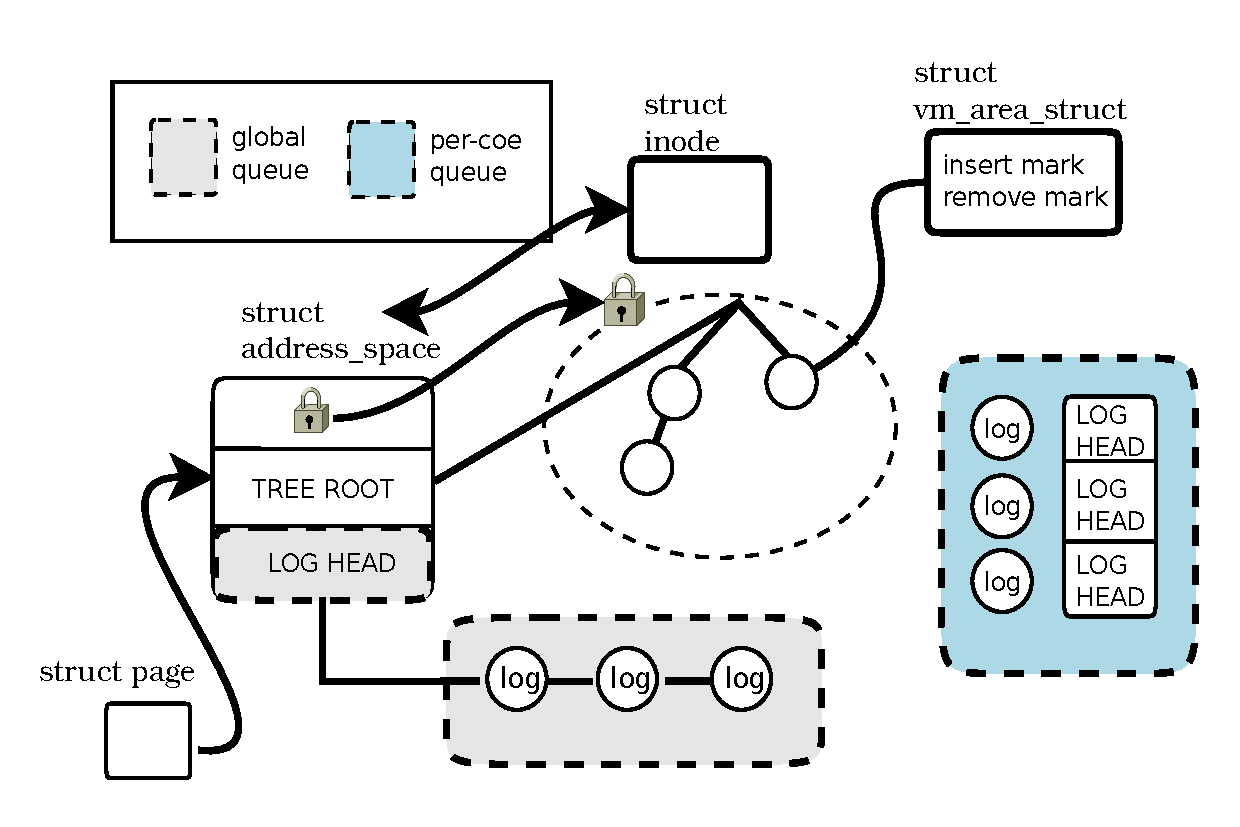
\includegraphics[width=0.5\textwidth]{fig/jaildocker}
  \end{center}
  \caption{Overview of towards a docker contrainer-based
  partitioning}
  \label{fig:basic}
\end{figure}

%$$$$$$$$$$$$$$$$$$$$$$$$$$$$$$$$$$$$$$$$$$$$$$$$$$$$$$$$$$$$$$$$$$$$$$$$$$$$$$$$
%$$$$$$$$$$$$$$$$$$$$$$$$$$$$$$$$$$$$$$$$$$$$$$$$$$$$$$$$$$$$$$$$$$$$$$$$$$$$$$$$
% 제안하는 구조 framework 설명
%$$$$$$$$$$$$$$$$$$$$$$$$$$$$$$$$$$$$$$$$$$$$$$$$$$$$$$$$$$$$$$$$$$$$$$$$$$$$$$$$
This section describes our vision that will accommodate the previous
mentioned design consideration.
Our proposed scalable partitioning framework is figure~\ref{fig:basic} with the
necessary features.
The left side of figure shows our proposed framework, and the right side of
figure shows isolated Docker containers and per-socket CPU with memory.

%The main components of the framwork are the decistion engine.
Decision engine is one of the most important features
since every partitioning regarding Spark system workers are based
on our decision engine component.
The basic function of the decision engine chooses whether or not the job
run on the Docker container.
The necessity of the auto-tuner is that performance scalability depending on partitioning
size commonly differs from each server architecture.
To maximized CPU utilization, the straggler monitor and core injector are needed
because straggler tasks prolong job completion times, so the
early finished CPUs should inject to other Docker containers which
contained the straggler tasks.

\begin{figure*}[tb]
    \centering
    \begin{subfigure}[b]{0.25\textwidth}
        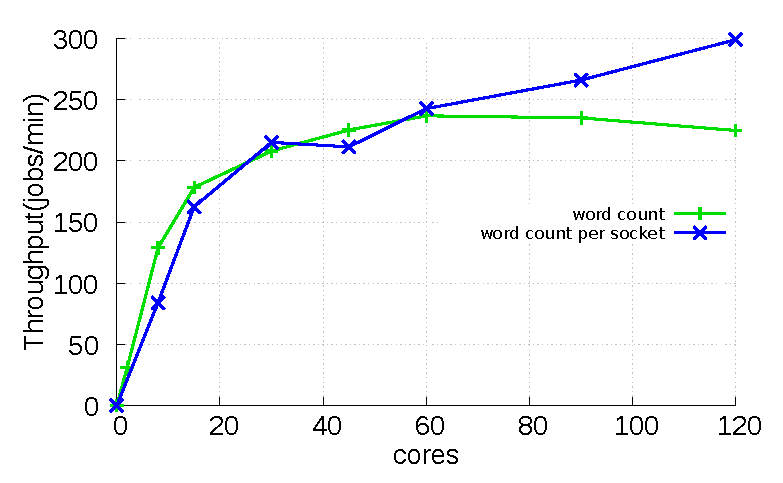
\includegraphics[width=1.8in]{graph/wc_docker.eps}
        \caption{Word Count}
    \end{subfigure}%
    \begin{subfigure}[b]{0.25\textwidth}
        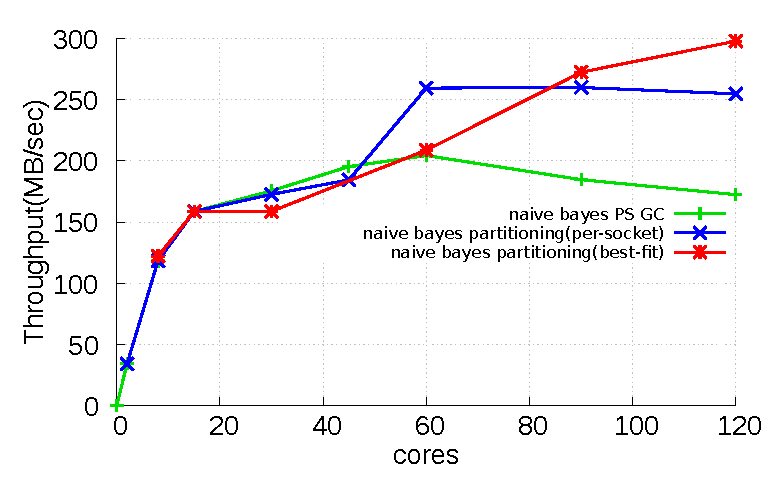
\includegraphics[width=1.8in]{graph/nb_docker.eps}
        \caption{Naive Basian}
    \end{subfigure}%
    \begin{subfigure}[b]{0.25\textwidth}
        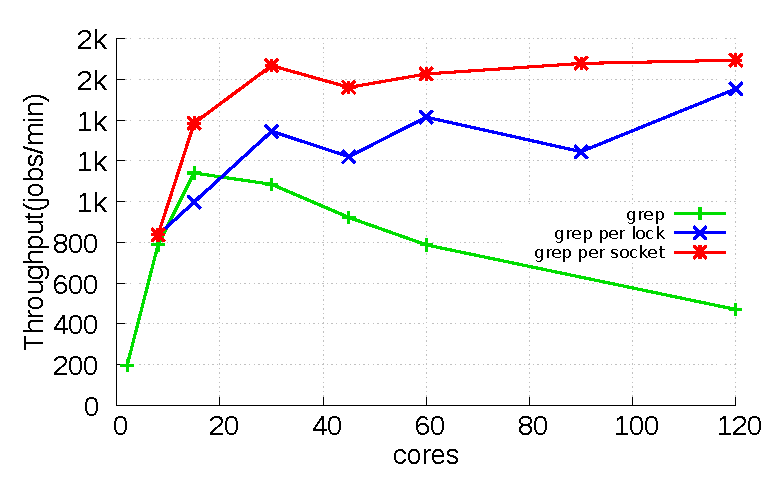
\includegraphics[width=1.8in]{graph/grep_docker.eps}
        \caption{Grep}
    \end{subfigure}%
    \begin{subfigure}[b]{0.25\textwidth}
        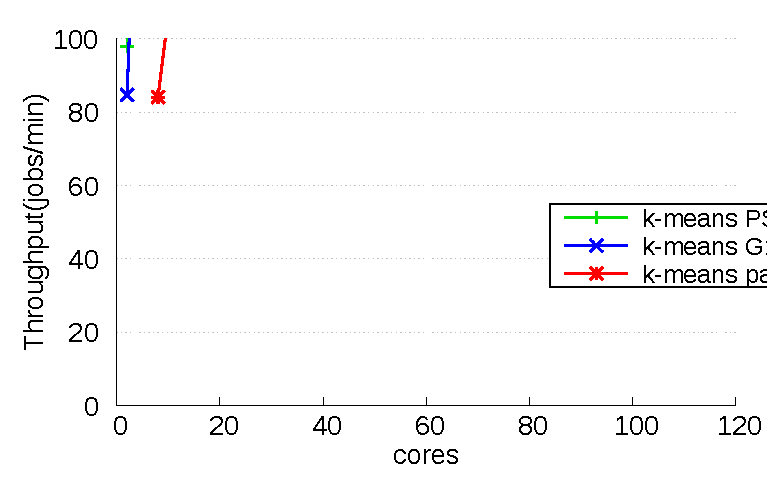
\includegraphics[width=1.8in]{graph/kmeans_docker.eps}
        \caption{K-means}
    \end{subfigure}%
    \caption{Performance scalability using docker container.}
    \label{fig:docker}
\end{figure*}


\begin{figure*}[tb]
    \centering
    \begin{subfigure}[b]{0.25\textwidth}
        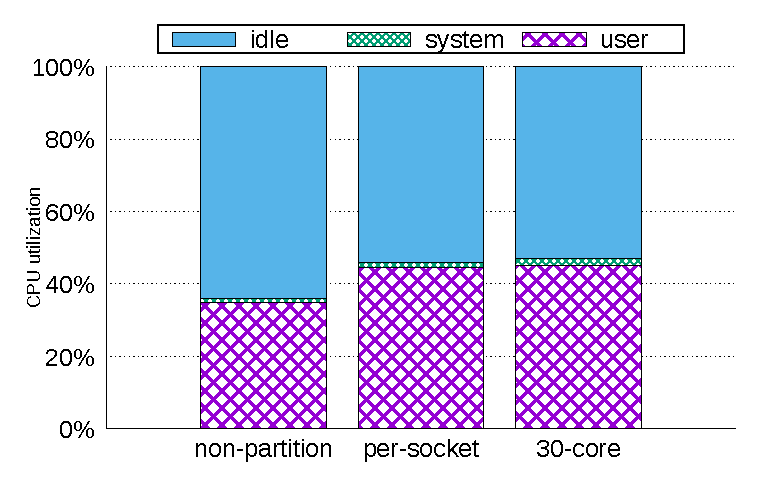
\includegraphics[width=1.8in]{graph/wc_cpuutils_docker.eps}
        \caption{Word Count}
    \end{subfigure}%
    \begin{subfigure}[b]{0.25\textwidth}
        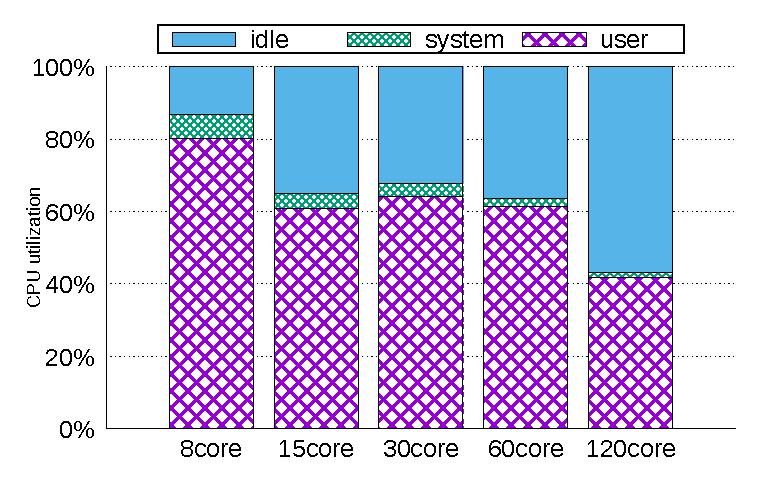
\includegraphics[width=1.8in]{graph/nb_cpuutils_docker.eps}
        \caption{Naive Basian}
    \end{subfigure}%
    \begin{subfigure}[b]{0.25\textwidth}
        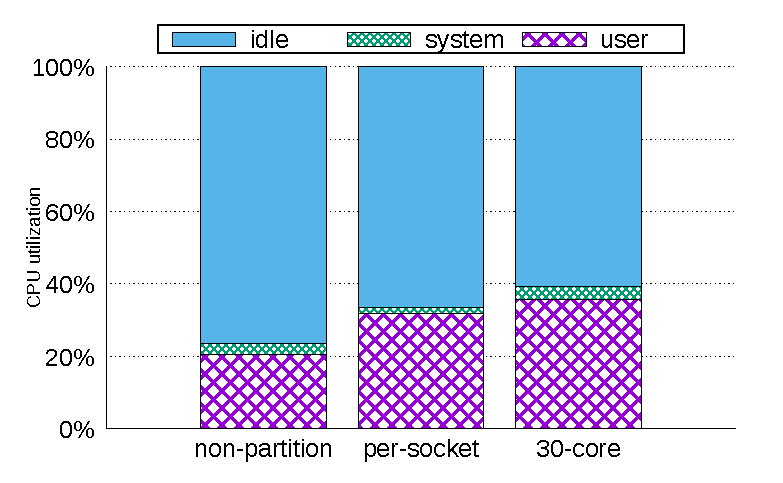
\includegraphics[width=1.8in]{graph/grep_cpuutils_docker.eps}
        \caption{Grep}
    \end{subfigure}%
    \begin{subfigure}[b]{0.25\textwidth}
        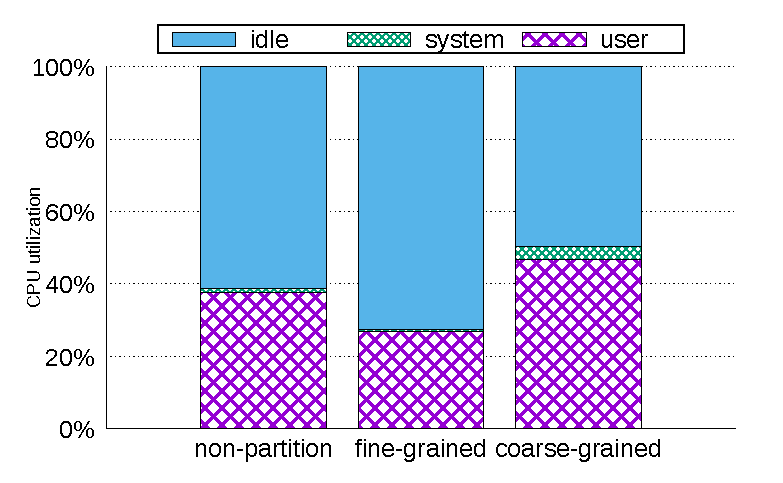
\includegraphics[width=1.8in]{graph/kmeans_cpuutils_docker.eps}
        \caption{K-means}
    \end{subfigure}%
        \centering
    \caption{CPU utilization on 120 core.}
    \label{fig:utilization2}
\end{figure*}
